\section{Gravitationally unstable disks} 
Gravitational instability (GI) becomes possible in a sufficiently
massive and/or cold disk. We explore how the emergence of GI affects
the MRI, and vice versa. To do so, we compute unstbale modes for  
isothermal disks with $Q < 0.2 $ ($Q_\mathrm{2D}\lesssim 0.67$) which
permits gravitational instability as well as the MRI.  

\subsection{Ideal disks}
We first consider ideal MHD by setting $\Lambda_0=100$ and $A=1$. 
Fig. \ref{compare_growth3} show growth rates for 
modes with $k_xH=1$ as a function of $\beta$ in disks with $Q=0.18$,
$Q=0.14$ and $Q=0.12$. The colorbar quantifies the importance of
self-gravity with 
\begin{align}
 \tau \equiv \frac{\avg{E_g}}{\avg{E_g} + \avg{E_m}}. 
\end{align} 
Thus, modes with $\tau  = 1$ are
energetically dominated by self-gravity (GI) and $\tau\ll1$ represents a mode
dominated by magnetic perturbations (MRI).  

All three cases display distinct GI modes (red/brown branch). The GI
growth rates are $\gamma\simeq 0.25\Omega,\,0.6\Omega,\,0.8\Omega$ for
$Q=0.18,\,0.14,\,0.12$, respecitvely. GI is stabilized by magnetic
pressure for sufficiently small $\beta$, and the critical field
strength increases with the self-gravity \citep{nakamura83}. For
$Q=0.18$, GI is stabilized for $\beta \lesssim 15$. Nevertheless, 
the MRI branch for $\beta < 15$ becomes self-gravitating, so that
density perturbations are still expected even though  GI does not
formally operate.  

%critical beta increases with $Q$

\begin{figure}
  \includegraphics[width=\linewidth,clip=true,trim=0cm 2.1cm 0cm
    0cm]{figures/compare_growth3_kx1_Q0d18.ps} 
  \includegraphics[width=\linewidth,clip=true,trim=0cm 2.1cm 0cm
    0.5cm]{figures/compare_growth3_kx1_Q0d14.ps} 
  \includegraphics[width=\linewidth,clip=true,trim=0cm 0cm 0cm
    0.5cm]{figures/compare_growth3_kx1_Q0d12.ps} 
  \caption{Growth rates for linear modes with $k_xH=1$ in an isothermal disk with
    $Q=0.18$ (top), $Q=0.14$ (middle) and $Q=0.14$ (bottom). The
    colorbar measures the importance of 
    self-gravity.  
    \label{compare_growth3}}
\end{figure}

The GI and MRI branches only interact when their growth rates
are similar. This is seen in Fig. \ref{compare_growth3} for $Q=0.18$
where the GI branch approaches an MRI branch at $\beta\simeq 25,\,
\gamma\simeq 0.2\Omega$. 
%Although the MRI is still most unstable, it is
%self-gravitating for $\beta\lesssim 50$ (uppermost curve). 
Some modes may have been missed in our
numerical search of eigenfrequencies. Thus, `breaks' along the
GI branch for $Q=0.18$ and $Q=0.12$ does not prove that the GI and MRI branches do not
intersect. However, the continous variation of $\tau$ with respect to
$\beta$ suggests that unstable modes can transition smoothly from
magnetically-dominated to gravitationally-dominated at low $\beta$.  

For $Q=0.12$ the GI growth rate exceeds all MRI modes. Notice the most
unstable MRI branch becomes self-gravitating for $20 \lesssim
\beta\lesssim 40$, but magnetic perturbations remain negligible
for GI. 
%we generally find MRI modes aquire significant potential
%perturbations but GI modes always have negligible magnetic
%perturbation. 
Fig. \ref{compare_growth3_Q01d2} show growth rates
as a function of $k_xH$ for the $Q=0.12,\,\beta=20$ disk. All
perturbations with $k_xH \lesssim 3.5$ are unstable. MRI operates on the largest
length scale, followed by GI at $0.7 \lesssim k_xH 1.7$. The 
transition between MRI to GI is smoother with increasing $k_xH$ as the
MRI becomes compressible. 

%Modes with $k_xH
% \gtrsim 1.7$ are neither pure MRI or GI. 
%GI wave lengths fit inside channel solutions 

\begin{figure}
  \includegraphics[width=\linewidth]{figures/compare_growth3_Q0d12_B20.ps}  
  \caption{Growth rates of unstable modes in the massive isothermal
    disk with $Q=0.12$ and $\beta=20$, as a function of the horizontal
    wavenumber $k_x$. The colorbar measures the importance of
    self-gravity. The solid line corresponds to MRI modes in the
    Cowling approximation. 
    \label{compare_growth3_Q01d2}}
\end{figure}


\subsection{Layered disks}
Can a disk with a dense, resistive midplane and a highly conducting
atmosphere  be subject to both MRI and GI but at different heights?  


%GI in the midplne and MRI in the surface? 
